%% This file was auto-generated by IPython.
%% Conversion from the original notebook file:
%% fem2.ipynb
%%
\documentclass[11pt,english,fleqn]{article}

%% This is the automatic preamble used by IPython.  Note that it does *not*
%% include a documentclass declaration, that is added at runtime to the overall
%% document.

\usepackage{amsmath}
\usepackage{amssymb}
\usepackage{graphicx}
\usepackage{ucs}
\usepackage[utf8x]{inputenc}

% needed for markdown enumerations to work
\usepackage{enumerate}

% Slightly bigger margins than the latex defaults
\usepackage{geometry}
\geometry{verbose,tmargin=3cm,bmargin=3cm,lmargin=2.5cm,rmargin=2.5cm}

% Define a few colors for use in code, links and cell shading
\usepackage{color}
\definecolor{orange}{cmyk}{0,0.4,0.8,0.2}
\definecolor{darkorange}{rgb}{.71,0.21,0.01}
\definecolor{darkgreen}{rgb}{.12,.54,.11}
\definecolor{myteal}{rgb}{.26, .44, .56}
\definecolor{gray}{gray}{0.45}
\definecolor{lightgray}{gray}{.95}
\definecolor{mediumgray}{gray}{.8}
\definecolor{inputbackground}{rgb}{.95, .95, .85}
\definecolor{outputbackground}{rgb}{.95, .95, .95}
\definecolor{traceback}{rgb}{1, .95, .95}

% Framed environments for code cells (inputs, outputs, errors, ...).  The
% various uses of \unskip (or not) at the end were fine-tuned by hand, so don't
% randomly change them unless you're sure of the effect it will have.
\usepackage{framed}

% remove extraneous vertical space in boxes
\setlength\fboxsep{0pt}

% codecell is the whole input+output set of blocks that a Code cell can
% generate.

% TODO: unfortunately, it seems that using a framed codecell environment breaks
% the ability of the frames inside of it to be broken across pages.  This
% causes at least the problem of having lots of empty space at the bottom of
% pages as new frames are moved to the next page, and if a single frame is too
% long to fit on a page, will completely stop latex from compiling the
% document.  So unless we figure out a solution to this, we'll have to instead
% leave the codecell env. as empty.  I'm keeping the original codecell
% definition here (a thin vertical bar) for reference, in case we find a
% solution to the page break issue.

%% \newenvironment{codecell}{%
%%     \def\FrameCommand{\color{mediumgray} \vrule width 1pt \hspace{5pt}}%
%%    \MakeFramed{\vspace{-0.5em}}}
%%  {\unskip\endMakeFramed}

% For now, make this a no-op...
\newenvironment{codecell}{}

 \newenvironment{codeinput}{%
   \def\FrameCommand{\colorbox{inputbackground}}%
   \MakeFramed{\advance\hsize-\width \FrameRestore}}
 {\unskip\endMakeFramed}

\newenvironment{codeoutput}{%
   \def\FrameCommand{\colorbox{outputbackground}}%
   \vspace{-1.4em}
   \MakeFramed{\advance\hsize-\width \FrameRestore}}
 {\unskip\medskip\endMakeFramed}

\newenvironment{traceback}{%
   \def\FrameCommand{\colorbox{traceback}}%
   \MakeFramed{\advance\hsize-\width \FrameRestore}}
 {\endMakeFramed}

% Use and configure listings package for nicely formatted code
\usepackage{listingsutf8}
\lstset{
  language=python,
  inputencoding=utf8x,
  extendedchars=\true,
  aboveskip=\smallskipamount,
  belowskip=\smallskipamount,
  xleftmargin=2mm,
  breaklines=true,
  basicstyle=\small \ttfamily,
  showstringspaces=false,
  keywordstyle=\color{blue}\bfseries,
  commentstyle=\color{myteal},
  stringstyle=\color{darkgreen},
  identifierstyle=\color{darkorange},
  columns=fullflexible,  % tighter character kerning, like verb
}

% The hyperref package gives us a pdf with properly built
% internal navigation ('pdf bookmarks' for the table of contents,
% internal cross-reference links, web links for URLs, etc.)
\usepackage{hyperref}
\hypersetup{
  breaklinks=true,  % so long urls are correctly broken across lines
  colorlinks=true,
  urlcolor=blue,
  linkcolor=darkorange,
  citecolor=darkgreen,
  }

% hardcode size of all verbatim environments to be a bit smaller
\makeatletter 
\g@addto@macro\@verbatim\small\topsep=0.5em\partopsep=0pt
\makeatother 

% Prevent overflowing lines due to urls and other hard-to-break entities.
\sloppy

\setlength{\mathindent}{0pt}
\setlength{\parindent}{0pt}
\setlength{\parskip}{8pt}
\begin{document}

Sınırlı Elementler Metodu (Finite Elements Method)

Bu metot differansiyel, kismi differansiyel denklemleri (partial
differential equations) yaklasiksal olarak modelleme ve cozmenin
yontemleridir.

Formul: Baslangic denklemi
\[ \frac{-d}{dx} \bigg( c(x) \ \frac{du}{dx} \bigg) = f(x) \]
Iki tarafi da $v(x)$ ile carpiyoruz ve 0 to 1 sinirlariyla entegralini
aliyoruz.
\[ \int_0^1 \frac{-d}{dx} \bigg( c(x) \ \frac{du}{dx} \bigg) v(x)dx = \int_0^1 f(x)v(x)dx \]
Parcali entegral (integration by parts) formulu soyledir:
\[ \int y \ dz = y  z \int z \ dy \]
Ana formulun bolumlerini, parcali entegrale gore bolusturursek:
\[ dz = \frac{-d}{dx} \bigg( c(x) \ \frac{du}{dx} \bigg) dx  \]\[ z = - c(x) \ \frac{du}{dx}  \]\[ y = v(x)  \]\[ dy = \frac{dv}{dx}dx \]
Yukarida $dz$ icinde $dx$ ve $\frac{1}{dx}$ birbirini iptal eder.
Parcali entegral formulunun sag tarafina gore yerlerine koyarsak:
\[ \int_0^1 v(x)dx \frac{-d}{dx} \bigg( c(x) \ \frac{du}{dx} \bigg) = - [v(x) c(x) \frac{du}{dx} \bigg]_{x=0}^{x=1} \int_0^1 c(x) \ \frac{du}{dx} \frac{dv}{dx}dx \]
Ustteki parcali entegral aciliminda sol taraf entegrale sinir degerleri
aldiginda, sag taraftaki $yz$ sonucunun ayni sinir degerlerine tabi
olduguna dikkat edelim.

Differansiyel denklemde sinir kosullari $x=1$ durumunda $c(1)u'(1)=0$,
ve $x=0$ durumunda $v(0)=0$ olarak biliniyor. O zaman ustteki denklemin
sol tarafinda $x=0$ ve $x=1$ kosullari icin tanimli bolum $0 - 0 = 0$
olacaktir ve denklemden atilabilir. Geriye kalanlar
\[ \int_0^1 c(x) \frac{du}{dx} \frac{dv}{dx} dx  = \int_0^1 f(x)v(x)dx \]
Bu fonksiyonu Galerkin adli bir matematikci bulmus, ``zayif form (weak
form)'' olarak adlandiriliyor.

Simdi diyelim ki n tane test fonksiyonu sectik $\phi_1(x),..,\phi(n)$ ve
bu fonksiyonlarin $U_j$ sayilari ile carpiminin toplamini, yani bir tur
kombinasyonunu $u(x)$ yerine kullanmaya karar verdik.
\[ U(x) = U_1 \phi_1+ ... + U_n\phi_n \]
O zaman
\[ U'(x) = U_1 \phi_1'+ ... + U_n\phi_n' \]\[ = \sum_1^n U_j \frac{d\phi_j}{dx} \]
Simdi $du / dx$ yerine $U'(x)$ koyarsak
\[ \int_0^1 c(x) \bigg( \sum_1^n U_j \frac{d\phi_j}{dx}\bigg)  \frac{dV_i}{dx} dx  = \int_0^1 f(x)V_i(x)dx \]
Dikkat edelim, $v(x)$ yerine $V_i(x)$ kullandik. Ustteki formul her i
icin yeni bir formul ``uretecek''. Niye $V_i$? Zayif formdaki $v(x)$
formulunu de zaten biz uydurmustuk, yani $v(x)$ biz ne istersek o olur.
O zaman bu fonksiyonu n tane formul uretmek icin bir numara olarak
kullaniliyoruz, n tane formul olunca matrisin n x n elemanini
doldurabilecegiz ve cozume erisebilecegiz. Ek not, cogunlukla $V_i(x)$
icin $\phi_i$ formulleri kullaniliyor.

Ayrica formuldeki $U_j$ kismini cekip cikartirsak ve bir vektor icine
koyarsak, geri kalanlar bir $K_{ij}$ matrisi icinde tutulabilir.
\[ K_{ij} = \int_0^1 c(x) \frac{d\phi_j}{dx} \frac{dV_i}{dx} dx  \]
Sag taraf ayni sekilde i tane formul uretir
\[ F_i = \int_0^1 f(x)V_i(x)dx \]
Final formul matrix formunda basit bir sekilde temsil edilebilecektir.
\[ KU = F \]
Ornek

Ornek olarak $-u'' = 1$ denklemini cozelim. Not: Differansiyel
denklemlerde sonuc bulmak demek bir ``fonksiyon'' bulmak demektir.
Normal cebirsel denklemlerde sonuc bulmak degiskenlerin ``sayisal''
degerini bulmak demektir. Birazdan bulacagimiz sonuc $u(x)$
``fonksiyonu'' olacak.

Eger denklem $-u''=1$ ise o zaman bu formulu ana forma uygun hale
getirmek icin $c(x) = 1$ olarak almamiz gerekir. $-u''=1$ denkleminde
esitligin sag tarafi 1 olduguna gore $f(x) = 1$ demektir.

Artik $\phi$ fonksiyonlarini secme zamani geldi. Bu fonksiyonlarin
``toplami'' hedefledigimiz fonksiyonu yaklasiksal (approximate) olarak
temsil edecek. Ornek olarak secebilecegimiz bir fonksiyon ``sapka
fonksiyonu (hat function)'' olarak bilinen ucgen fonksiyonlar olabilir.
Alttaki figurde bu fonksiyonlari goruyoruz.

\begin{codecell}
\begin{codeinput}
\begin{lstlisting}
im=imread("fem_hat.png"); imshow(im)
\end{lstlisting}
\end{codeinput}
\begin{codeoutput}
\begin{verbatim}
<matplotlib.image.AxesImage at 0xb04834c>
\end{verbatim}
\begin{center}
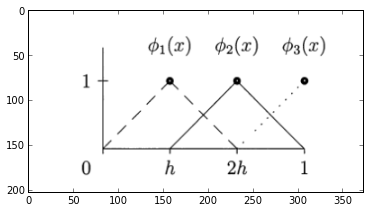
\includegraphics[width=0.7\textwidth]{fem2_files/fem2_fig_00.png}
\par
\end{center}
\end{codeoutput}
\end{codecell}
Bu figurde x ekseninin h buyuklugundeki parcalara bolundugunu goruyoruz.

Entegralleri hesaplayalim
\[ F_1 = \int_0^1 V_1(x)dx \]
Daha once $V_1$ ve $\phi_1$'i ayni kabul ettigimizi belirtmistik.

Yukaridaki entegralin aslinda bir alan hesabi yaptigini goruyoruz.
Sinirlar $0$ ve $1$ arasinda, ama $2h$ otesinde zaten $\phi_1$
fonksiyonu yok. $\phi_1$'in alani nedir? Alan ucgenin alani: Taban carpi
yukseklik bolu 2: $2h$, yuksekligi $1$, o zaman alan
$(2h \times 1) / 2 = 1/3$

Benzer mantikla bakarsak, $F_2$ ile $F_1$ ayni, yani $1/3$. $F_3$ ise
onlarin yarisi, yani $1/6$.

$K_{ij}$ nasil hesaplanacak? $c(x) = 1$ oldugu icin formulden
cikarilabilir ve $V_1$ ve $\phi_1$'in ayni olduguna soyledik:
\[ K_{ij} = \int_0^1 c(x) \frac{d\phi_j}{dx} \frac{dV_i}{dx} dx \]\[ K_{11} = \int_0^1 \bigg( \frac{dV_1}{dx} \bigg) ^2 dx  \]
$dV_1/dx$ nedir? Birinci sapka fonksiyonunun turevidir. Bu tureve
bakarsak, $0$ ve $h$ arasinda arti egim (slope) $1/h$, $h$ ve $2h$
arasinda eksi egim $-1/h$ oluyor. Ama kare aldigimiz icin sonuc ayni,
$1/h^2$. O zaman h = 1/3 olduguna gore $1/(1/3)^2$, yani $dV_1/dx = 9$.
\[ K_{11} = \int_0^{2/3} 9 dx = 9x \ \bigg|_0^{2/3} = (9)(2/3) - 0 = 6 \]
$K_{22}$ seklen ayni fonksiyon parcasini temel aldigi icin ayni degere
sahip: 6. $K_{33}$ onlarin yarisi, esittir 3.

$K_{12}$ farkli egimlerin carpimi anlamina gelir, yani $V_1'$ ile $V_2'$
carpimi olur. Bu iki fonksiyona bakalim, 0 ile h arasinda $V_2$ yok,
egim 0. Ikisinin de sifir olmadigi, carpimda kullanilabilecek bir
egiminin oldugu tek aralik h ve 2h arasi. Burada $V_1' = -3, V_2 = 3$.
\[ K_{12} = \int_{1/3}^{2/3} (3)(-3) dx = -9x \bigg|_{1/3}^{2/3} = -6 - (-3) = -3 \]
Ayni sekilde $K_{23} = -3$. Ama $K_{13} = 0$ cunku hic cakisma yok.

Matrisi doldurursak,
\[
KU = F
\]\[
\begin{bmatrix}
    6 & -3 & 0 \\
    -3 & 6 & -3 \\
    0 & -3 & 3     
\end{bmatrix}
\begin{bmatrix}
    U_1 \\
    U_2 \\
    U_3
\end{bmatrix} =
\begin{bmatrix}
    1/3 \\
    1/3 \\
    1/6
\end{bmatrix}
 \]
Python kodu

\begin{codecell}
\begin{codeinput}
\begin{lstlisting}

import numpy as np
K = [[6., -3., 0],
     [-3., 6., -3.],
     [0., -3., 3.]]

f = [1./3., 1./3., 1./6.]

print np.linalg.solve(K,f)

\end{lstlisting}
\end{codeinput}
\begin{codeoutput}
\begin{verbatim}
[ 0.27777778  0.44444444  0.5       ]
\end{verbatim}
\end{codeoutput}
\end{codecell}
\begin{codecell}
\begin{codeinput}
\begin{lstlisting}
print 5./18., 4./9., 1./2.
\end{lstlisting}
\end{codeinput}
\begin{codeoutput}
\begin{verbatim}
0.277777777778 0.444444444444 0.5
\end{verbatim}
\end{codeoutput}
\end{codecell}
Rapor edilen degerler bu denklemin bilinen cozumu
$u(x) = x - \frac{1}{2}x^2$ ile 0, h, 2h noktalarinda (mesh points)
birebir uyum gosterdigini goruyoruz. Yani yaklasiksal olarak
differansiyel denklemi cozmeyi basardik.

Kaynaklar

Strang, G., Computational Science and Engineering, 2007

\end{document}
